\chapter{Literature Review}\label{chapter:Literature Review}


\section{\gls{OPF} Objective Functions}
Typical objectives in \gls{OPF} are summarized in \cite{yang2023optimal}: generation cost minimization, transmission loss minimization, and carbon emission minimization. Moreover, \cite{chen2012optimal} consider not only generation cost but also \gls{EV} charging cost in the \gls{EV}-aware \gls{OPF} problem. On the other hand, \cite{andrianesis2020distribution} take marginal cost of active and reactive power, and transformer degradation cost into account. Furthermore, multi-objective formulation can be found in the related research (\cite{duman2021symbiotic, paul2024multi}).


\section{\gls{OPF} Constraints}
The classical \gls{OPF} formulation, as introduced by \cite{carpentier1962contribution}, includes power flow balance equations and various operational limits, such as line loading limits, bus voltage limits, and generator output limits \cite{yang2018fundamental}. Depending on the specific application, additional constraints may also be integrated. For instance, \cite{nikkhah2020stochastic} develop an \gls{OPF} framework that incorporates renewable energy, \gls{BESS}, and \gls{EV} charging stations. In their model, beyond the traditional \gls{OPF} constraints, they also include constraints for wind and solar energy generation output, spinning reserve requirements, \gls{BESS} charging, and \gls{EV} charging capacity. Similarly, \cite{paul2024multi} present a multi-objective \gls{OPF} model that integrates \gls{V2G} technology, incorporating \gls{EV} discharging and charging rate limitations as additional constraints.


\section{Optimization Methods for \gls{OPF} Problems}
The \gls{OPF} problem has been a significant and extensively studied non-linear optimization challenge since the 1960s. Consequently, numerous methods have been developed to address \gls{OPF} in the research community. The initial \gls{OPF} solution, introduced by \cite{Dommel1968}, is formulated as a continuous \gls{NLP} problem. They employ gradient adjustment algorithms to achieve a near-optimal solution, as the control parameters did not require higher accuracy than what could be adjusted and measured in the actual system. However, traditional \gls{NLP} is both computationally and theoretically challenging, with many methods only guaranteeing locally optimal solutions (\cite{wei1998interior}). Consequently, numerous modified formulations have been developed and have gained popularity.\\
\cite{nejdawi2000efficient} convert the OPF into a \gls{SQP} problem, a type of \gls{NLP} method. \gls{SQP} is an iterative method for nonlinear optimization where the original nonlinear problem is approximated by a sequence of quadratic programming subproblems. They also apply \gls{IPM} to solve the subproblem for each iteration. Each subproblem then optimizes a quadratic model of the objective function subject to linearized constraints, making \gls{SQP} particularly effective for solving large-scale constrained nonlinear optimization problems.\\
Other popular reformulations of \gls{OPF} are \gls{SOCP} (\cite{jabr2006radial, marley2016solving, Kayacik2021, chowdhury2023second}) and \gls{SDP} (\cite{bai2008semidefinite, lavaei2011zero, madani2014convex, madani2015promises}), both of which are classified under convex relaxation. \gls{SOCP} involves linear and second-order (quadratic) cone constraints by approximating non-linear power flow equations with quadratic constraints. \cite{marley2016solving} claim deploying \gls{SOCP} relaxation for initialization can help achieving convergence faster and reduce the likelihood of reaching local optimum. \cite{chowdhury2023second} propose \gls{SOCP}-\gls{OPF} model with coupling coefficients to address the mutual coupling effects on the unbalanced AC lines. \cite{Kayacik2021}'s work shows the potential of \gls{SOCP} lies in scalability and small optimality gap.\\
On the other hand, \gls{SDP} is an optimization framework where the constraint can be formulated as an affine combination of symmetric matrices remains positive semidefinite. Compared to \gls{SOCP}, \gls{SDP} provides a more accurate representation of non-linear power flow equations using semidefinite constraints. Nonetheless, \gls{SDP} solvers require more computational time than \gls{SOCP} (\cite{lavaei2011zero}). Moreover, \cite{lesieutre2011examining} demonstrates through a numerical optimal power flow example that a non-zero duality gap can arise in the \gls{SDP} formulation as a line-flow inequality constraint is progressively tightened, leading the SDP to fail in providing a physically meaningful solution to the original \gls{OPF} problem. Nonetheless, \cite{madani2014convex} discovered that when \gls{SDP} relaxation fails to provide an exact solution, it typically still yields a low-rank solution that is computationally efficient and reveals important underlying structures, making it valuable for practical applications.
%For instance, \cite{nikkhah2020stochastic} proposed relaxed mixed-integer non-linear programming to solve the \gls{OPF} problem in the micro-grid application.


\section{(Deep) \acrlong{RL}}
Traditionally, the power system is dispatched by an alternating current \gls{OPF} solver within 15-minute to one-hour intervals. Considering highly fluctuated power generation and load consumption, a faster solution to the non-convex \gls{OPF} is needed for real-time applications. Approaches such as \gls{NLP}, \gls{SQP}, \gls{SOCP} are time-intensive for reaching convergence when implemented on large power networks. Moreover, since these methods do not possess learning components, optimization iterations are needed for every new load and generation profile, making them computationally expensive. They are unable to adapt to the stochasticity of the optimization environment that contains unpredictable load profiles, grid tariff and renewable energy generation. Thus, their applications are limited in real-world cases.\\ 
One effective approach to addressing the complexity and dynamic nature of \gls{OPF} is to implement \gls{DRL} algorithm. \acrfull{RL} is a type of machine learning where an agent learns to make decisions by interacting with an uncertain environment to maximize cumulative rewards through trial and error (\cite{sutton2018reinforcement}). \acrfull{DRL} refers to \gls{RL} with agents as \gls{DNN}. \gls{DRL} algorithms excel in complex decision-making processes, making them highly suitable for addressing non-linearity and stochasticity in power systems (\cite{zhang2019deep, chen2022reinforcement}). Given the dynamic nature of power systems, \gls{DRL} agents can adapt to changing conditions, learning optimal control strategies in real time through continuous interaction with the environment and updating their policies based on new observations and feedback. Another main advantage of \gls{DRL} is that although it transforms the challenging optimization problem into a series of matrix multiplications online with the cost of lengthy offline training, leading to a significant speed-up of several orders of magnitude.\\ % main advantages: dynamics and time
Before delving into \gls{DRL} methods applied to \gls{OPF}, it's essential to cover some fundamental concepts of \gls{RL}. The first topic introduced is the \gls{MDP}, which provides the formal framework for environments in \gls{RL} and is discussed in subsection \ref{subsec:MDP}. Following that, the subsections \ref{subsec:model-free} and \ref{subsec:A-C} cover the concepts of model-free \gls{RL} and Actor-Critic, as these are crucial components of the predominant \gls{RL} algorithms used in the \gls{OPF} applications.


\subsection{\acrfull{MDP}} \label{subsec:MDP}
 \acrfull{MDP} is characterized by state space \gls{symb:S}, action space \gls{symb:A}, transition probability function \gls{symb:P}, mapping a state-action pair $(s,a) \in $ \gls{symb:S} $\times$ \gls{symb:A} to a distribution on the state space, and reward function \gls{symb:R} (\cite{bellman1957markovian,kaelbling1996reinforcement,sutton2018reinforcement}). As illustrated in Figure \ref{fig:MDP}, the action $a_{t} \in$ \gls{symb:A} is selected by the agent based on the policy $\pi(a_{t}|s_{t})$ and the reward $R_{t} = R(s_{t},a_{t})$ is sent back to the agent. Meanwhile, through the transition probability function \gls{symb:P}, the next state $s_{t+1} \in$ \gls{symb:S} is determined.
\begin{figure}[h!]
\begin{center}
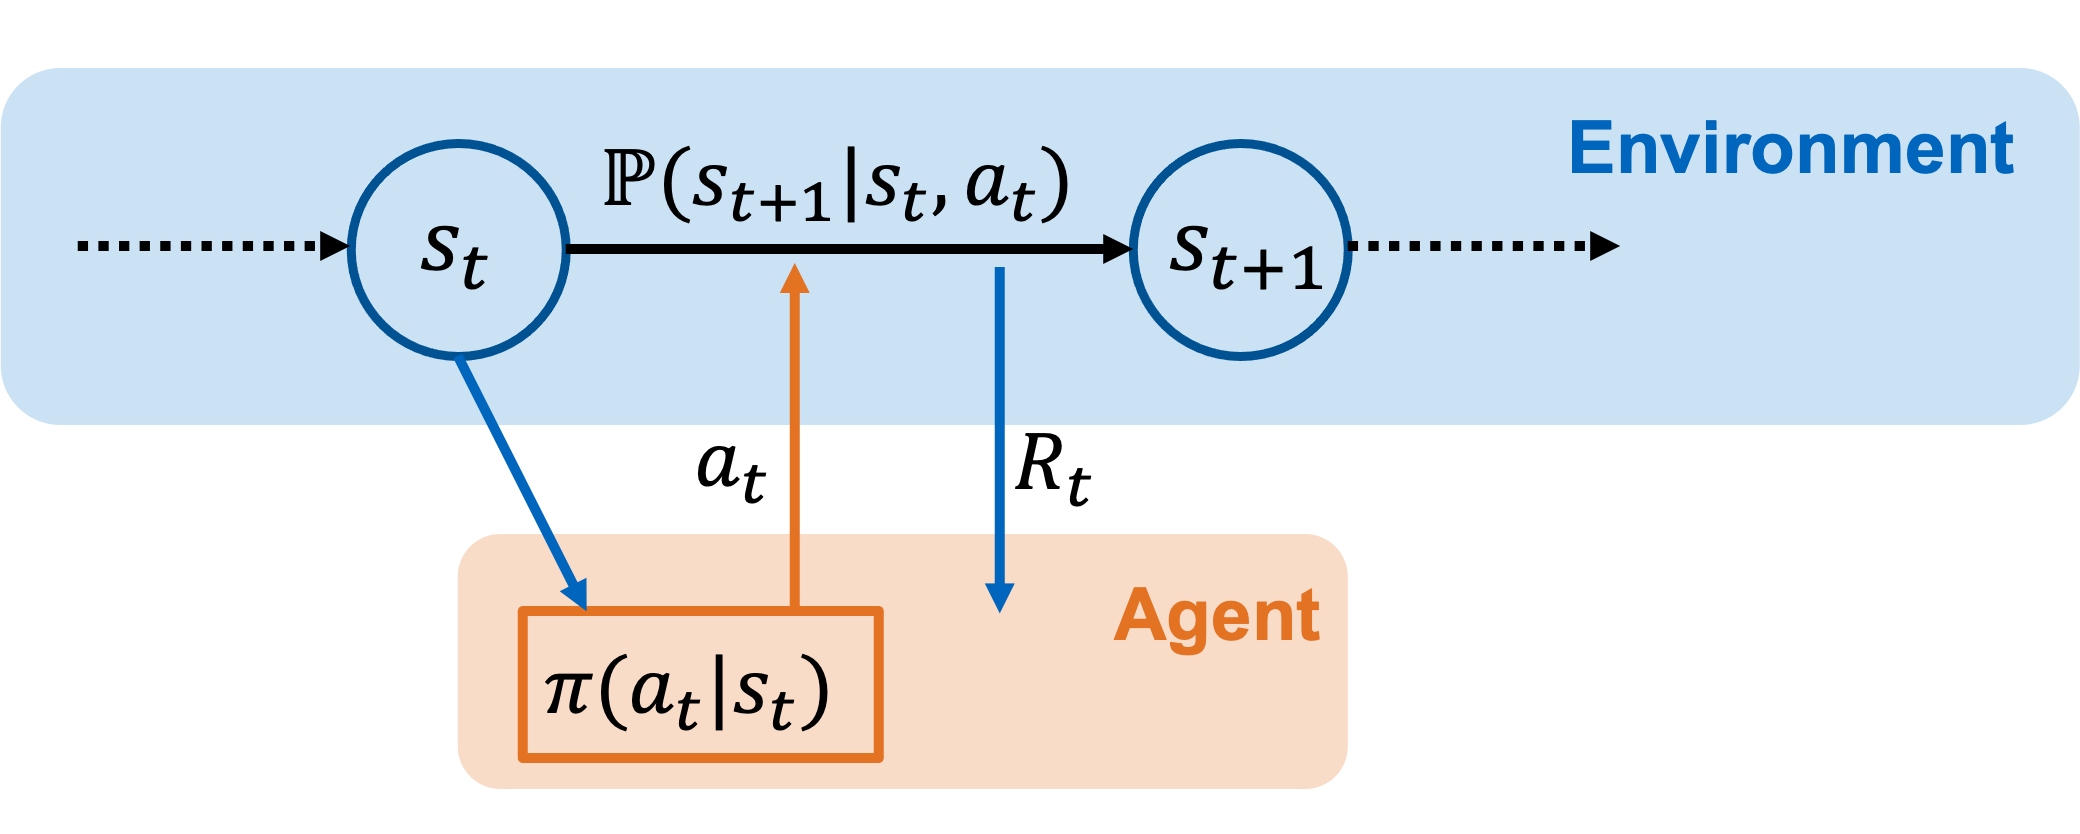
\includegraphics[width=0.9\textwidth]{LaTeX_Vorlagen_Studienarbeiten/images/MDP Framework.png}
\caption{Framework of \acrlong{MDP} (\cite{chen2022reinforcement})}
\label{fig:MDP}
\end{center}
\end{figure}
This process continues through the following time steps, forming the so-called Markov Chain. The ultimate goal is to decide an optimal policy $\pi^{*}$ that maximizes the value of a state $V^{*}(s)$. This value represents the expected infinite discounted sum of rewards that the agent will accumulate if it begins in that state and follows the optimal policy $\pi^{*}$, with the discount rate $\gamma$ that penalizes the rewards in the future.
\begin{equation*}
    V^{*}(s)=\underset{\pi}{max} \mathbb{E}\Bigl( \sum_{t=0}^{\infty}\gamma^{t}R_{t}\Bigr)
\end{equation*}
The optimal value $V^{*}(s)$ can also be expressed as the sum of the expected instantaneous reward $R(s,a)$ and the expected discounted value of the next state $s'$, assuming the agent takes the best available action $a$ (\cite{kaelbling1996reinforcement}).
\begin{equation*}
    V^{*}(s)=\underset{a}{max}\Bigl( R(s,a)+\gamma\sum_{s' \in S}\mathbb{P}(s,a,s')V^{*}(s')\Bigr), \forall s \in S
\end{equation*}
Given the optimal value function, the optimal policy can be expressed as (\cite{kaelbling1996reinforcement})
\begin{equation*}
    \pi^{*}(s)=\underset{a}{argmax}\Bigl( R(s,a)+\gamma\sum_{s' \in S}\mathbb{P}(s,a,s')V^{*}(s')\Bigr), \forall s \in S.
\end{equation*}
Dynamic programming methods for \gls{MDP}, such as value iteration algorithm and policy iteration algorithm requires known reward function \gls{symb:R} and transition probability function \gls{symb:P} to find the optimal policy (\cite{bertsekas2012dynamic}). On the contrary, a \gls{RL} agent can learn with the past observations by interacting with the environment without knowing the reward function and transition probability function. 


\subsection{Model-Free \acrlong{RL}}\label{subsec:model-free}
\gls{RL} methods can be categorized into model-based \gls{RL} and model-free \gls{RL}. The former aims to learn the model, that is, both \gls{symb:R} and \gls{symb:P}. Even though it is more sample efficient, it can be complex to develop and can introduce computational overhead (\cite{wang2019benchmarking, moerland2023model}). Whereas the model-free \gls{RL} approach does not necessitate to learn the accurate model. Instead, policy or value function is learned. Hence, it is more robust and less computationally expensive (\cite{koryakovskiy2017benchmarking,swazinna2022comparing}). Since robustness is critical in real life when solving \gls{OPF}, this work aims at model-free \gls{RL}. Model-free \gls{RL} can be further categorized into two types: value-based and policy based. Value-based methods focus on learning value functions, i.e. $V(s)$ and the optimal policy is derived indirectly from these value functions. One typical value-based method is Q-Learning , of which the "Q" stands for action-value function $Q(s,a)$, representing the expected cumulative reward the agent receives by taking action $a$ in state $s$ (\cite{tsitsiklis1994asynchronous}). By updating $Q(s,a)$ at each iteration, optimal policy can be determined when reaching convergence. This algorithm is straightforward. Nonetheless, it becomes computationally infeasible when the complexity of the environment rises or the action space is continuous because storing large amount of Q-values and updating a Q-value for each state-action pair are required (\cite{das2012improved}). Contrary to value-based methods, policy-based methods can handle high-dimensional or continuous action spaces. It is because the policy that the agent aims to learn can be represented as a probability distribution. Since  continuous action space is involved in most of the \gls{OPF} problems, policy-based and hybrid methods, such as Actor-Critic, that combine strengths of both value-based and policy based approaches are more suitable for solving the \gls{OPF}.


\subsection{Actor-Critic Framework}\label{subsec:A-C}
Compared to policy-based and other hybrid methods, the Actor-Critic methods together with \gls{DNN} build a relatively popular framework for \gls{OPF} because it offers a flexible and efficient approach to handling the complexity, non-linearity, and high dimensionality inherent in \gls{OPF} tasks (\cite{arwa2020reinforcement, chen2022reinforcement, massaoudi2023navigating}). The Actor-Critic framework with \gls{DNN} involves an Actor network that learns to take actions and a Critic network that evaluates these actions, with both components iteratively improving through feedback loops (\cite{konda1999actor}). As depicted in the Figure \ref{fig:A-C}, the Actor network takes the current state $s$ as input and outputs the action $a$ based on a policy $\pi(a|s;\theta)$ where $\theta$ is denotes the weights of the policy or Actor network. The environment responds with a new state $s'$ and reward $R$. The Critic estimates the action-value function $V(s)$ by taking the action $a$ selected by the Actor and state $s$ as input. Given the discount factor $\gamma$, the Critic updates its network weights $w$ based on the \gls{TD} error, which can be written as:
\begin{equation*}
    \delta = R + \gamma V(s') - V(s).
\end{equation*}
The Actor then updates $\theta$ in the direction suggested by the Critic's feedback, gradually improving the policy.
\begin{figure}[h!]
\begin{center}
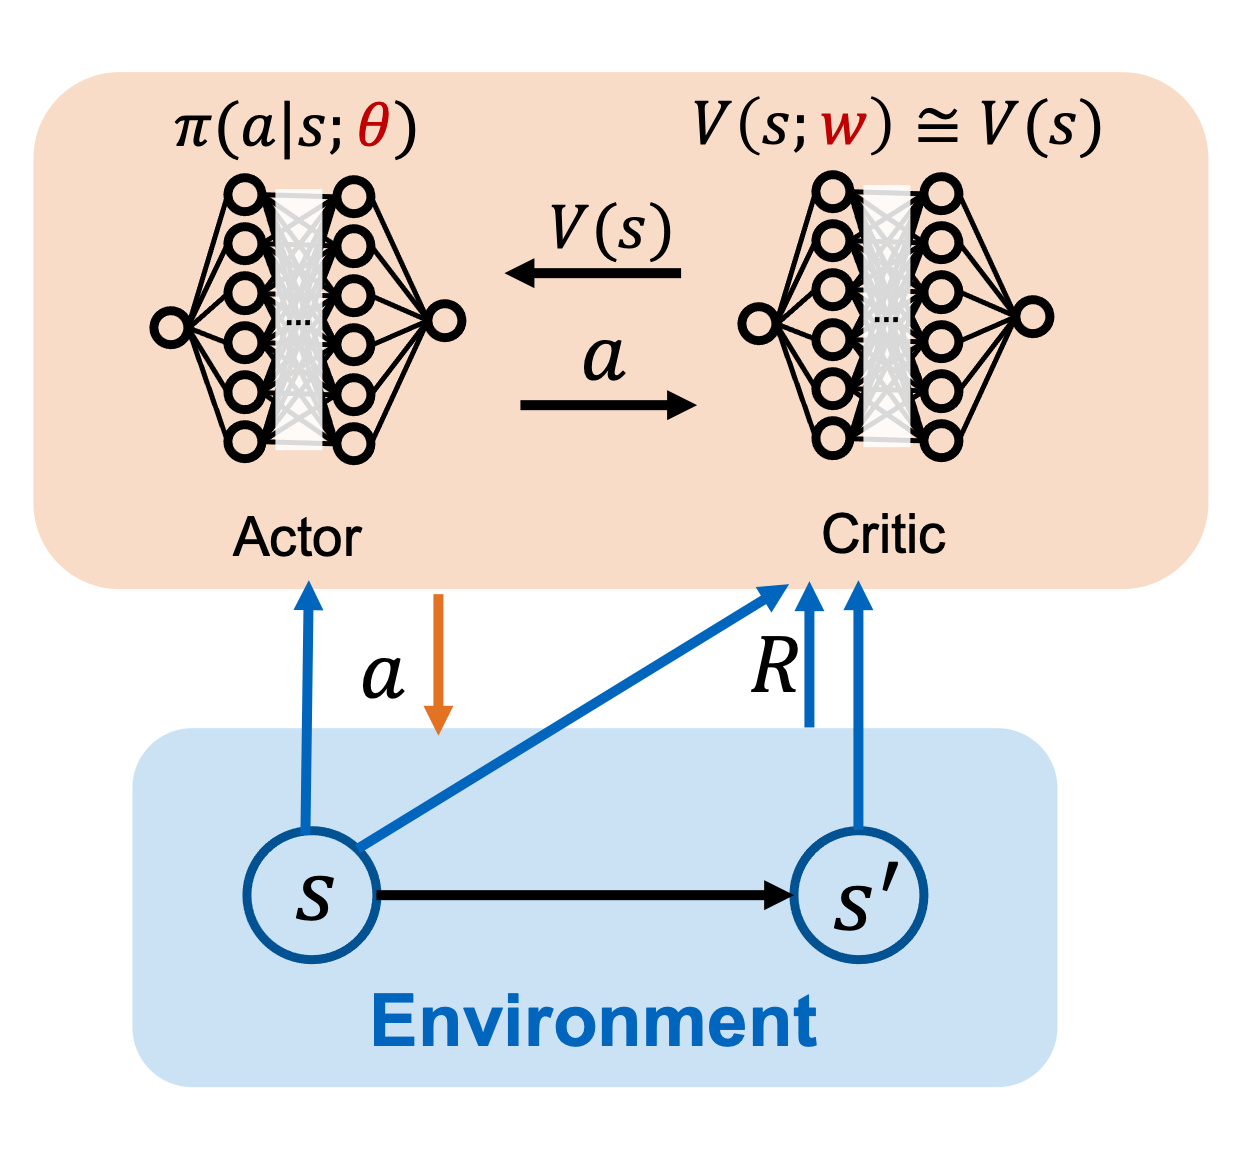
\includegraphics[width=0.8\textwidth]{LaTeX_Vorlagen_Studienarbeiten/images/A-C Framework.png}
\caption{Actor-Critic Framework}
\label{fig:A-C}
\end{center}
\end{figure}


\subsection{\acrlong{DRL} Application for \gls{OPF} Problems}\label{subsec:DRLApplication}
With the rising popularity of artificial intelligence, \gls{DRL} has gained attention in power system application (\cite{arwa2020reinforcement, chen2022reinforcement, massaoudi2023navigating}). For economic dispatch or \gls{OPF} problems, \gls{DRL} agents determine the optimal output of generation units to meet demand at the lowest cost, while satisfying all operational constraints. For instances, \cite{yan2020real} implement \gls{DDPG} algorithm (\cite{lillicrap2015continuous}), an Actor-Critic algorithm designed for continuous action spaces, for \gls{OPF}. Instead of the Critic network, they utilize \gls{IP} method to derive the deterministic policy gradient of a Lagrangian-based value function. Additionally, \cite{zhen2022design} chose \gls{TD3} algorithm (\cite{fujimoto2018addressing}) for solving \gls{OPF} problem. \gls{TD3} algorithm is an improvement over \gls{DDPG} that addresses some of the instability issues in training by doubling Critic networks. Due to the use of twin Critics and delayed updates, it is more complex and has high computational costs. Thus, another alternative, \gls{PPO} algorithm (\cite{schulman2017proximal}), becomes one of the most commonly used approach among the literature. The benefits of using \gls{PPO} are low computational overhead and simple implementation, leading to faster convergence (\cite{massaoudi2023navigating}). \cite{cao2021deep} deploy \gls{PPO} algorithm in an environment simulating \gls{BESS}-integrated power system to solve the multi-period \gls{OPF} problem and claim that their approach is promising in the real-time operation. 
Several works also suggest using behavior cloning for initialization of the policy or Actor network in order to enhance the training performance of \gls{PPO} (\cite{zhou2020data,zhou2021deep,feng2024safe}). Other algorithms, such as \gls{SAC} (\cite{haarnoja2018soft}), also demonstrate promising training performance and results (\cite{sayed2022feasibility}). 

%TODO: add reward function of OPF use cases